\chapter{Introduction}
\label{sec:introduction}

During the past decades, robotics has evolved from the heavy industrial manipulators, that worked only to a very specific structured environment doing specific repetitive tasks, to mobile robots that navigate themselves to unstructured environments and they are able to perform a variety of tasks. A particular field of robotics that has gained a lot of attention lately, is localization and motion of the mobile robot based only on information coming from its own sensors, and particularly its cameras.

The reason for choosing cameras as the main source of information in modern robotics, and as in our specific case to an MAV, is that they provide an abundance of information while their weight, power consumption and price is considerably less compared to other kinds of sensors, such as laser scanners. Furthermore, nowadays exist advanced computer vision algorithms that allow us to robustly extract the necessary information and of course the proper hardware that allows the on board and fast processing of the acquired data.  

Furthermore, the scientific interest regarding autonomous mobile robots, is strongly attracted to low weight multi rotor MAVs. Some of their merits over conventional designs, such as fixed wing platforms, are their ability for vertical take off and landing, they can hover over specific areas as long as their energy source allows and their ability to perform tight maneuvers in confined spaces. Their wide commercial availability combined with their reduced prices makes them a very attractive platform for experimentation. Their uses, which are rapidly increasing, include parcel delivery, inspection of structures, search and rescue operations and of course use by hobbyists for various other tasks.     

In this project, the AscTec's Firefly MAV is used, to present the realization of the MAV's high level control only with the use of visual commands. Thus, the MAV uses only the data available from its onboard sensors to deduce its desired pose in the three dimensional world based on the user's visual commands. These commands are given by the Apriltag markers. First the whole system was build in simulation, using the RotorS simulator created by the ASL \cite{RotorsSimulator} and then the developed algorithms were evaluated in the real system. 


\section{Summary}
\label{sec:summary}

In \autoref{sec:SystemDescription} is a thorough system description, providing information about the visual markers, the MAV used and the frame analysis of the system. In \autoref{sec:SystemSetup}, comes the setup of the system, explaining the various packets written in order to make the system run in simulation. In \autoref{sec:ExperimentalResults}, there will be presented the experimental results both from the simulated and the real system. Finally in \autoref{sec:cocnlusion} we present the conclusions along with some ideas about what could be done in the future. 
 
 
\section{Related Work}
\label{sec:related_work}

In the recent years, many teams have been able to perform various kinds of motions with the MAVs (\cite{5509452},\cite{hehIFAC11},\cite{trajectoryGenerationAndControl}, \cite{dandreaTedTalk}), but all of them heavily relied on the use of external motion capture systems (VICON\protect\footnotemark), in order to obtain localization data and their maneuvers are generally predefined. Other teams, have used Apriltags\cite{olson2011tags} for providing localization data to their robots. Such examples are \cite{lafaroLab} and \cite{robornSwam}, they use them to provide localization data in ground vehicles with different configurations, in the first case the Apriltags are statically attached to the ceiling of the lab while in the latter are attached on the robots and on the walls of the lab. At the Carnegie Mellon team \cite{robornSwam}, their use is to provide both relative localization among the ground vehicles but also providing absolute localization information from the static located markers. Furthermore, in \cite{lingkevin2014} and \cite{schaves-2015a} they use the aforementioned markers in order to land the MAVs towards, static or moving landing sights. Other uses of the marker include  \cite{hoogervorst2015bsc} where they were used to compensate sensor loss in a different MAV by providing its 6 DOF pose estimate based on the marker detection and in \cite{6842304} where it augments the localization data and compensates the IMU data drift. \\

\begin{figure}
	\centering
	 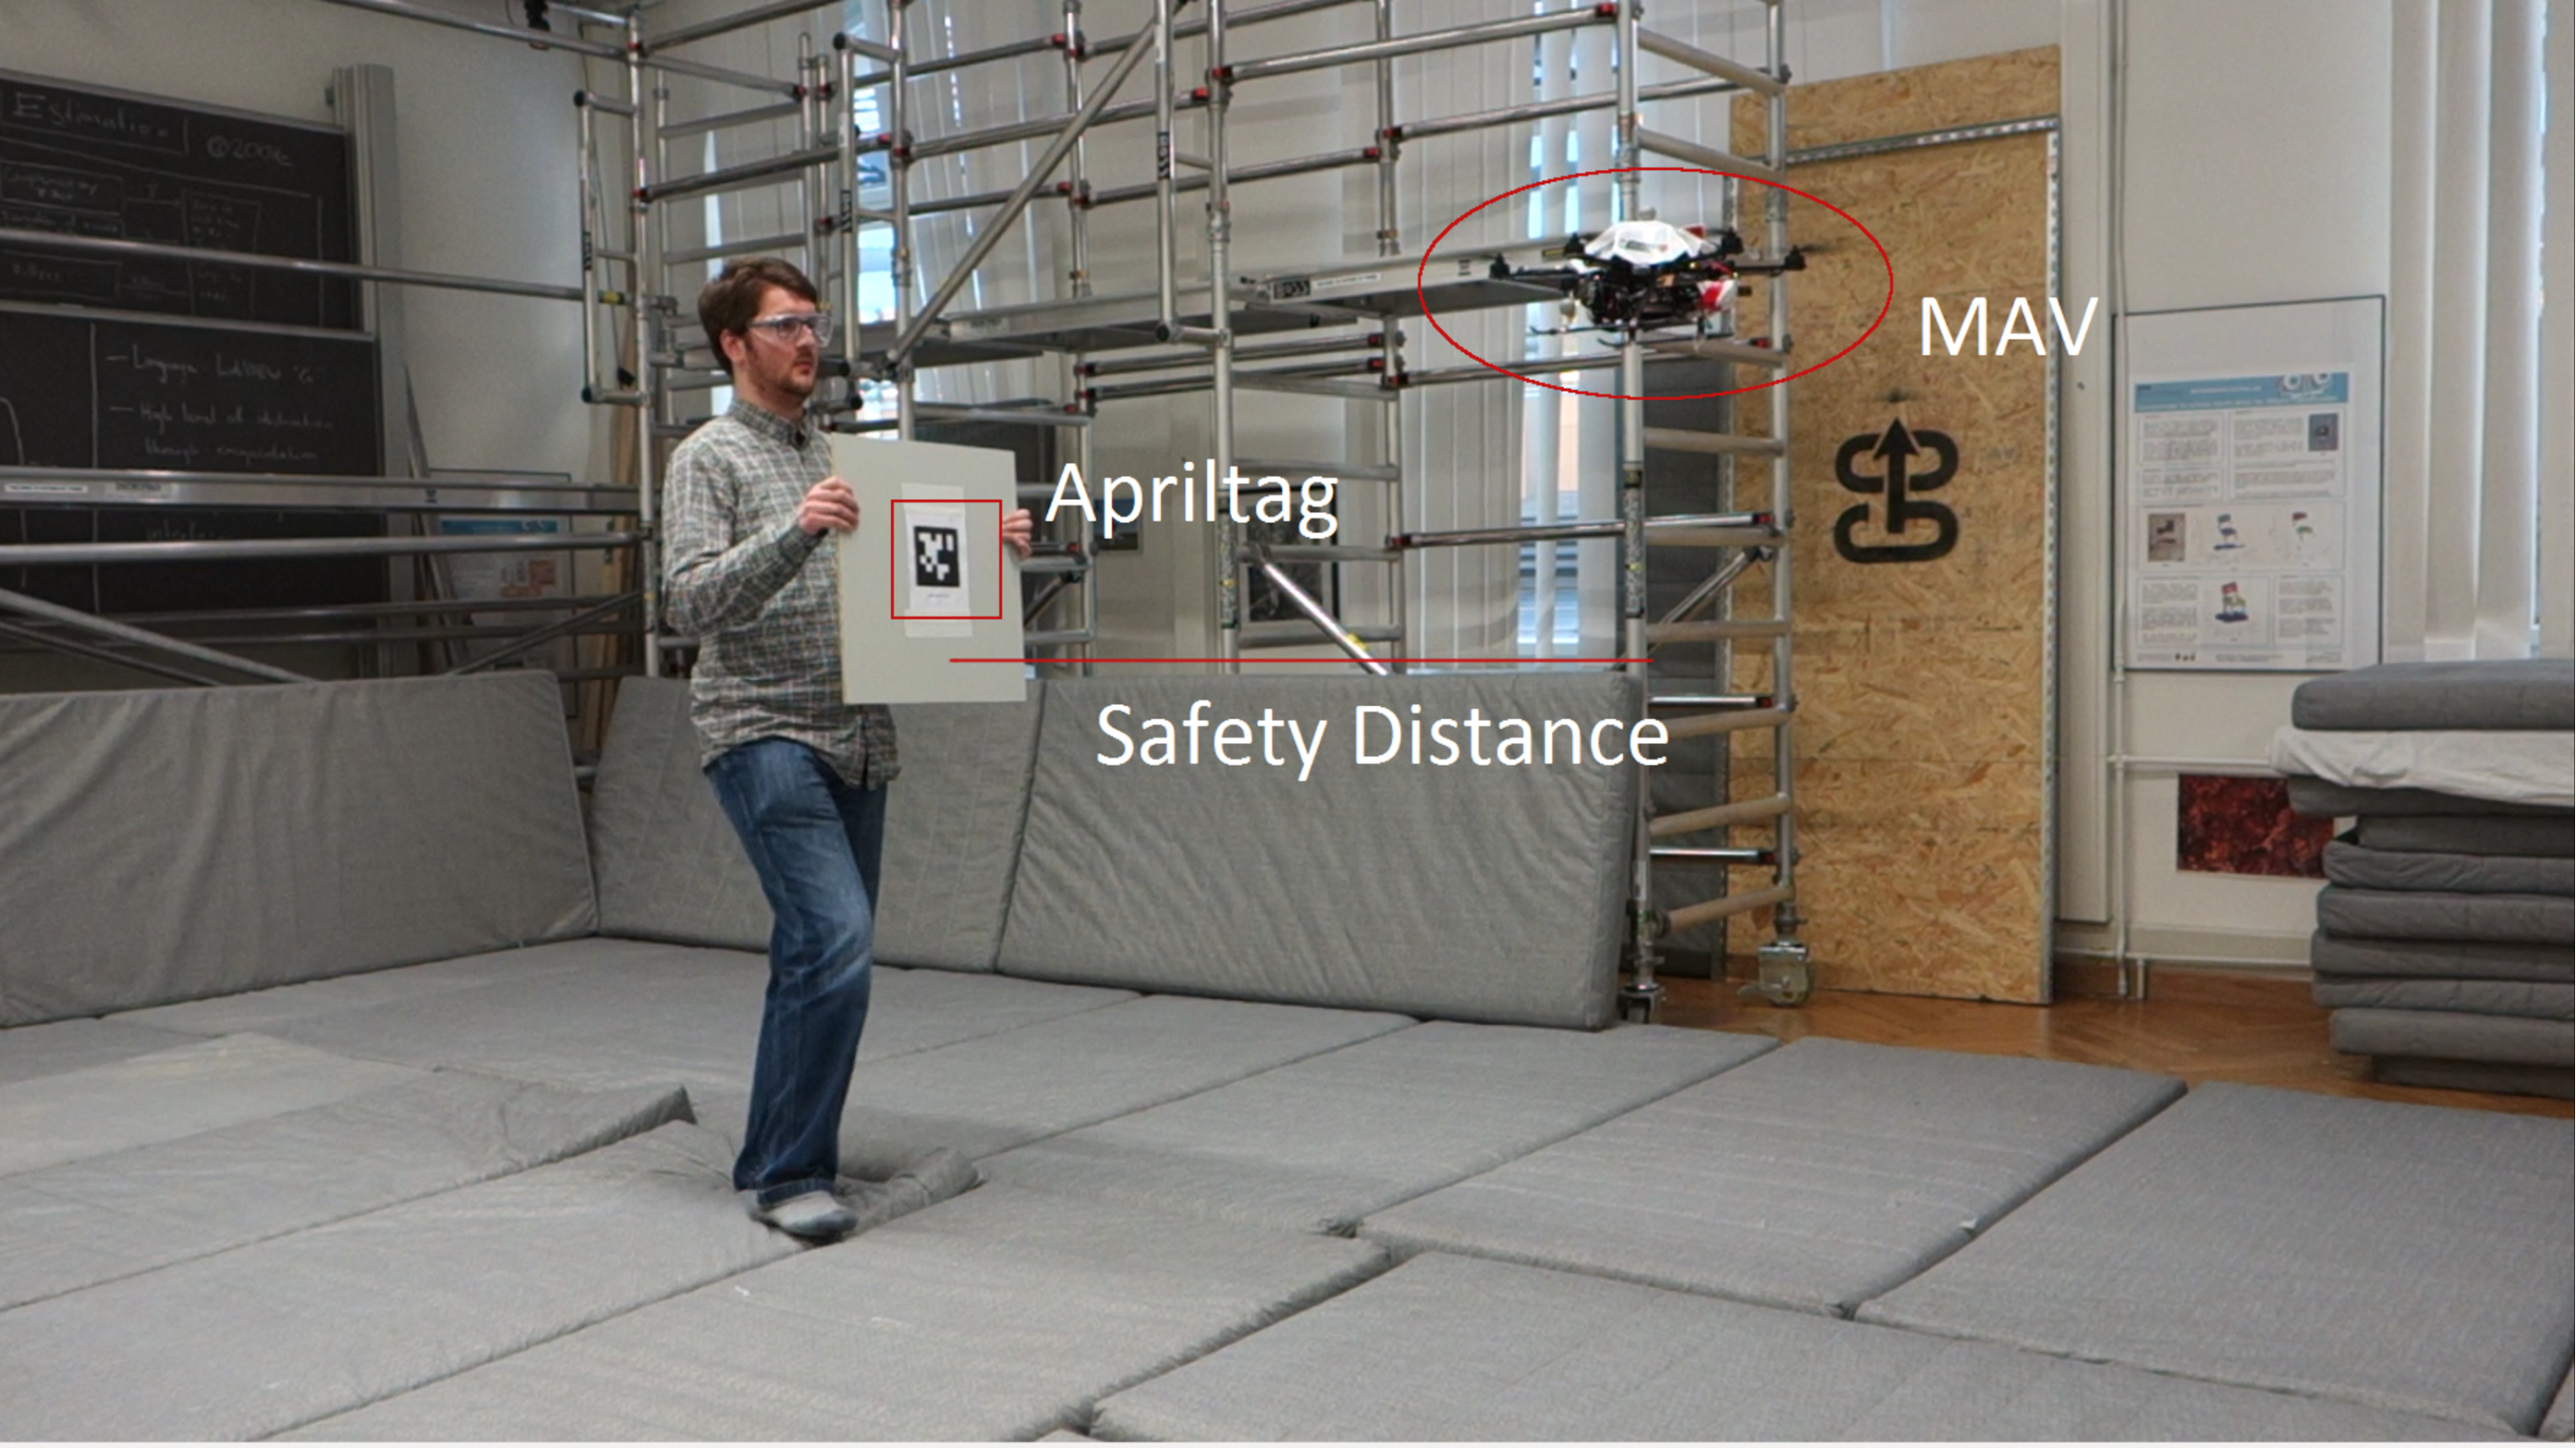
\includegraphics[width=1.00\textwidth]{images/real_experiment_v1.pdf}
	 \caption{The MAV detects the marker and moves to the desired position, based on the marker detection}
	 \label{pics:experimentCapture}
\end{figure}

In our case, we wanted a system that would be able to provide information that would allow us to follow the visual commands presented by the user and also ensure that there will be adequate distance between the user and the MAV, as presented in figure \ref{pics:experimentCapture}. Thus, we also used the Apriltag markers. Our approach differs form the aforementioned, since we don't use an external motion capture system in order to decide the MAV's desired position. The markers are not statically attached to the ceiling or to the lab's walls, the markers are held by the user and they can be moved without limitations, as long as they stay in the camera's field of view. Furthermore, our system is able to land anywhere just by presenting the proper marker to the MAV and finally we do not use the Apriltags in order to compensate or substitute sensor mistakes or loss. It can be easily seen, that the advantages of our approach are the fact that we do not rely on any external system, for the marker detection and desired position estimation, our system is highly versatile, we don't use any static landmarks and we can land at any place the user wants. Of course, there are some disadvantages too.  First of all, the precision and resolution of our system, is much lower compared to systems using VICON. Furthermore, the unconstrained motion of the marker leads sometimes to the loss of the marker's detection, since the Apriltag can get out of the camera's field of view. Last but not least, the ability of the MAV to land whenever the user commands it, may lead to problematic situations in cases where the user chooses poorly the landing position.


  
\footnotetext{http://www.vicon.com}
  
  
  
  
  
  


